\documentclass[conference]{IEEEtran}
\IEEEoverridecommandlockouts
% The preceding line is only needed to identify funding in the first footnote. If that is unneeded, please comment it out.
\usepackage{cite}
\usepackage{amsmath,amssymb,amsfonts}
\usepackage{algorithmic}
\usepackage{graphicx}
\usepackage{textcomp}
\usepackage[portuguese]{babel}
\usepackage[utf8]{inputenc}
\usepackage{hyperref}
\def\BibTeX{{\rm B\kern-.05em{\sc i\kern-.025em b}\kern-.08em
    T\kern-.1667em\lower.7ex\hbox{E}\kern-.125emX}}
\begin{document}

\title{Unscramble Me - The Game
}

\author{\IEEEauthorblockN{1\textsuperscript{st} Michael Pacheco}
\IEEEauthorblockA{\textit{Universidade Federal de Ouro Preto} \\
\textit{Campus Morro do Cruzeiro}\\
Ouro Preto, Brasil \\
pacheco@decom.ufop.br}
\and
\IEEEauthorblockN{2\textsuperscript{nd} Alex Sandro Sobreira de Paula}
\IEEEauthorblockA{\textit{Universidade Federal de Ouro Preto} \\
\textit{Campus Morro do Cruzeiro}\\
Ouro Preto, Brasil \\
alexsspop89@yahoo.com}
\and
\IEEEauthorblockN{3\textsuperscript{rd} Eduardo Aguiar Martins}
\IEEEauthorblockA{\textit{Universidade Federal de Ouro Preto} \\
\textit{Campus Morro do Cruzeiro}\\
Ouro Preto, Brasil \\
eduagmart@gmail.com}
}

\maketitle

\begin{abstract}
O objetivo deste documento é apresentar a arquitetura de um jogo eletrônico chamado Unscramble Me. Este jogo será desenvolvido na disciplina de Redes de Computadores (BCC361) ministrada pelo docente Saul Emanuel Delabrida Silva, da Universidade Federal de Ouro Preto.
\end{abstract}

\begin{IEEEkeywords}
jogo, redes, sockets, thread, servidor
\end{IEEEkeywords}

\section{Introdução}
Unscramble Me é um jogo \textit{multiplayer online} cujo objetivo dos jogadores é desembaralhar corretamente uma palavra gerada pelo servidor. O primeiro jogador que conseguir desembaralhar corretamente a palavra, vencerá.

\section{Funcionamento}

Ao abrir o jogo, o jogador - agora chamado cliente - tentará conectar-se ao servidor. Após uma conexão bem sucedida o cliente deverá fornecer um nome de usuário / apelido e selecionar uma das seguintes opções:

\begin{enumerate}
\item Criar sala
  \begin{enumerate}
  \item Iniciar partida
  \item Sair da sala
  \item Sair do jogo
  \end{enumerate}

\item Entrar em uma sala já existente
  \begin{enumerate}
  \item Sair da sala
  \item Sair do jogo
  \end{enumerate}

\item Sair do jogo
\end{enumerate}

\section{Arquitetura do Sistema}
O sistema está dividido em duas partes: cliente e servidor.
A comunicação cliente-servidor se dá por meio de sockets.
Ao iniciar a aplicação o cliente tentará comunicar-se com o servidor. Caso a comunicação falhe a aplicação terminará. Caso contrário o servidor aceitará a requisição de conexão e iniciará uma \textit{thread} que ficará responsável por receber mensagens deste cliente.
Após uma comunicação bem sucedida, a aplicação do cliente instanciará duas \textit{threads}, uma responsável por receber e outra por enviar mesagens ao servidor. A figura \ref{fig:sysarch} ilustra a arquitetura básica do sistema.

\begin{figure}[ht]
\caption{System architecture}
\centering
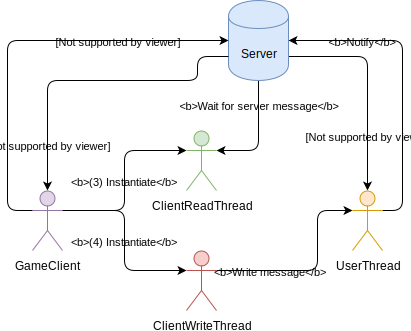
\includegraphics[width=250px]{images/Architecture}
\setlength{\abovecaptionskip}{15px}
\label{fig:sysarch}
\end{figure}


\section{Regras}
\begin{enumerate}
\item Um jogador deve criar uma sala ou entrar em uma já existente para poder participar de uma partida.
\item Uma sala deve conter pelo menos 5 jogadores para que a partida possa iniciar.
\item Apenas o host da sala pode iniciar uma partida.
\item Uma partida termina quando há um vencedor ou quando o tempo limite de 5 minutos for atingido.
\item Não há um limite de jogadores por sala.
\item O primeiro jogador que conseguir desembaralhar corretamente a palavra, dentro do tempo limite, vencerá o jogo.
\item Não é permitido entrar em uma partida que já está em andamento.
\end{enumerate}

\begin{thebibliography}{00}
\bibitem{b1} Code Java, How to Create a Chat Console Application in Java using Socket. 20 December 2017. \url{http://www.codejava.net/java-se/networking/how-to-create-a-chat-console-application-in-java-using-socket}
\end{thebibliography}

\end{document}